\documentclass[1p]{elsarticle_modified}
%\bibliographystyle{elsarticle-num}

%\usepackage[colorlinks]{hyperref}
%\usepackage{abbrmath_seonhwa} %\Abb, \Ascr, \Acal ,\Abf, \Afrak
\usepackage{amsfonts}
\usepackage{amssymb}
\usepackage{amsmath}
\usepackage{amsthm}
\usepackage{scalefnt}
\usepackage{amsbsy}
\usepackage{kotex}
\usepackage{caption}
\usepackage{subfig}
\usepackage{color}
\usepackage{graphicx}
\usepackage{xcolor} %% white, black, red, green, blue, cyan, magenta, yellow
\usepackage{float}
\usepackage{setspace}
\usepackage{hyperref}

\usepackage{tikz}
\usetikzlibrary{arrows}

\usepackage{multirow}
\usepackage{array} % fixed length table
\usepackage{hhline}

%%%%%%%%%%%%%%%%%%%%%
\makeatletter
\renewcommand*\env@matrix[1][\arraystretch]{%
	\edef\arraystretch{#1}%
	\hskip -\arraycolsep
	\let\@ifnextchar\new@ifnextchar
	\array{*\c@MaxMatrixCols c}}
\makeatother %https://tex.stackexchange.com/questions/14071/how-can-i-increase-the-line-spacing-in-a-matrix
%%%%%%%%%%%%%%%

\usepackage[normalem]{ulem}

\newcommand{\msout}[1]{\ifmmode\text{\sout{\ensuremath{#1}}}\else\sout{#1}\fi}
%SOURCE: \msout is \stkout macro in https://tex.stackexchange.com/questions/20609/strikeout-in-math-mode

\newcommand{\cancel}[1]{
	\ifmmode
	{\color{red}\msout{#1}}
	\else
	{\color{red}\sout{#1}}
	\fi
}

\newcommand{\add}[1]{
	{\color{blue}\uwave{#1}}
}

\newcommand{\replace}[2]{
	\ifmmode
	{\color{red}\msout{#1}}{\color{blue}\uwave{#2}}
	\else
	{\color{red}\sout{#1}}{\color{blue}\uwave{#2}}
	\fi
}

\newcommand{\Sol}{\mathcal{S}} %segment
\newcommand{\D}{D} %diagram
\newcommand{\A}{\mathcal{A}} %arc


%%%%%%%%%%%%%%%%%%%%%%%%%%%%%5 test

\def\sl{\operatorname{\textup{SL}}(2,\Cbb)}
\def\psl{\operatorname{\textup{PSL}}(2,\Cbb)}
\def\quan{\mkern 1mu \triangleright \mkern 1mu}

\theoremstyle{definition}
\newtheorem{thm}{Theorem}[section]
\newtheorem{prop}[thm]{Proposition}
\newtheorem{lem}[thm]{Lemma}
\newtheorem{ques}[thm]{Question}
\newtheorem{cor}[thm]{Corollary}
\newtheorem{defn}[thm]{Definition}
\newtheorem{exam}[thm]{Example}
\newtheorem{rmk}[thm]{Remark}
\newtheorem{alg}[thm]{Algorithm}

\newcommand{\I}{\sqrt{-1}}
\begin{document}

%\begin{frontmatter}
%
%\title{Boundary parabolic representations of knots up to 8 crossings}
%
%%% Group authors per affiliation:
%\author{Yunhi Cho} 
%\address{Department of Mathematics, University of Seoul, Seoul, Korea}
%\ead{yhcho@uos.ac.kr}
%
%
%\author{Seonhwa Kim} %\fnref{s_kim}}
%\address{Center for Geometry and Physics, Institute for Basic Science, Pohang, 37673, Korea}
%\ead{ryeona17@ibs.re.kr}
%
%\author{Hyuk Kim}
%\address{Department of Mathematical Sciences, Seoul National University, Seoul 08826, Korea}
%\ead{hyukkim@snu.ac.kr}
%
%\author{Seokbeom Yoon}
%\address{Department of Mathematical Sciences, Seoul National University, Seoul, 08826,  Korea}
%\ead{sbyoon15@snu.ac.kr}
%
%\begin{abstract}
%We find all boundary parabolic representation of knots up to 8 crossings.
%
%\end{abstract}
%\begin{keyword}
%    \MSC[2010] 57M25 
%\end{keyword}
%
%\end{frontmatter}

%\linenumbers
%\tableofcontents
%
\newcommand\colored[1]{\textcolor{white}{\rule[-0.35ex]{0.8em}{1.4ex}}\kern-0.8em\color{red} #1}%
%\newcommand\colored[1]{\textcolor{white}{ #1}\kern-2.17ex	\textcolor{white}{ #1}\kern-1.81ex	\textcolor{white}{ #1}\kern-2.15ex\color{red}#1	}

{\Large $\underline{12a_{0936}~(K12a_{0936})}$}

\setlength{\tabcolsep}{10pt}
\renewcommand{\arraystretch}{1.6}
\vspace{1cm}\begin{tabular}{m{100pt}>{\centering\arraybackslash}m{274pt}}
\multirow{5}{120pt}{
	\centering
	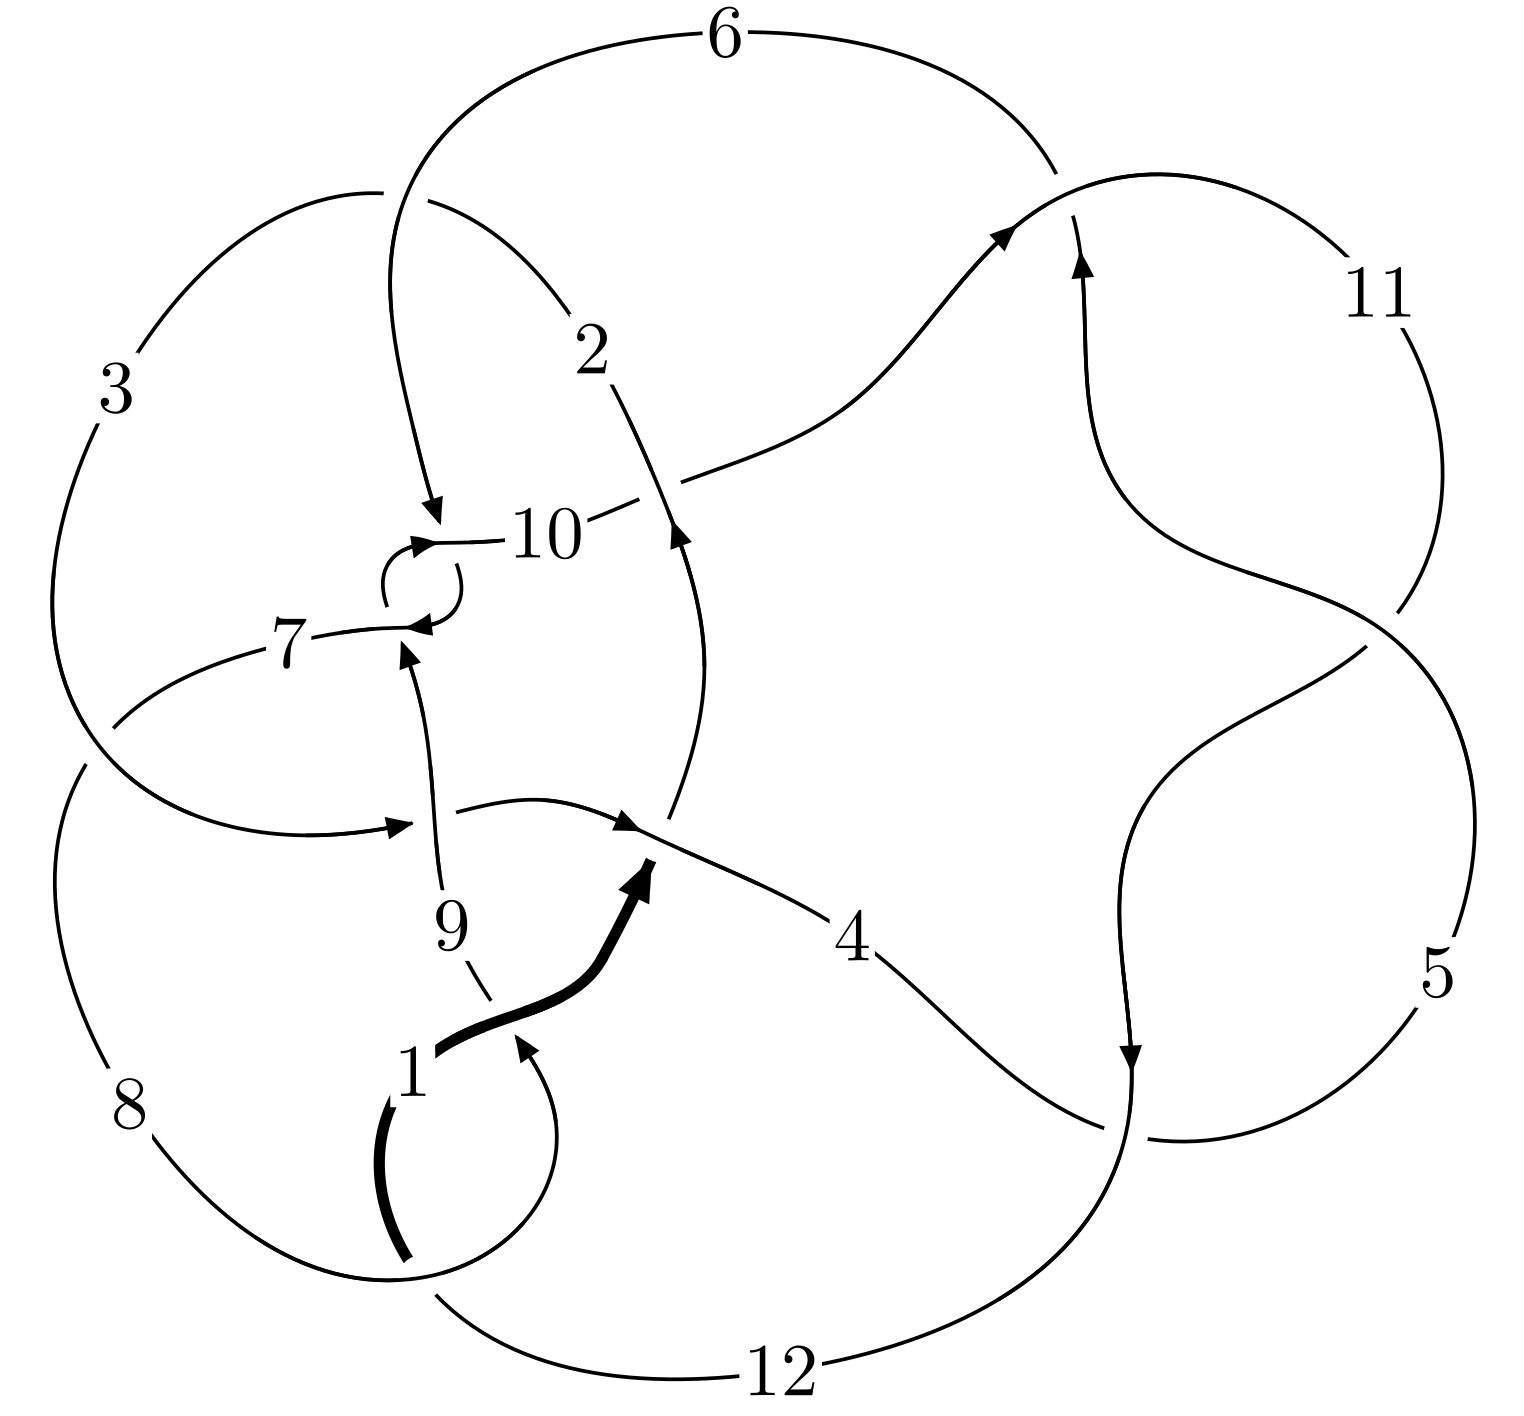
\includegraphics[width=112pt]{../../../GIT/diagram.site/Diagrams/png/1737_12a_0936.png}\\
\ \ \ A knot diagram\footnotemark}&
\allowdisplaybreaks
\textbf{Linearized knot diagam} \\
\cline{2-2}
 &
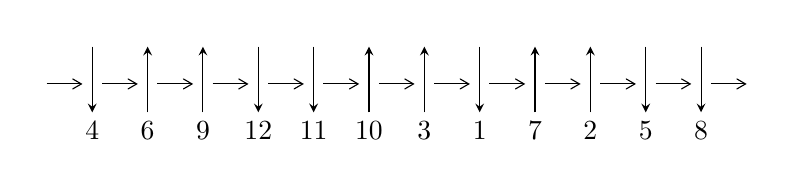
\begin{tikzpicture}[x=20pt, y=17pt]
	% nodes
	\node (C0) at (0, 0) {};
	\node (C1) at (1, 0) {};
	\node (C1U) at (1, +1) {};
	\node (C1D) at (1, -1) {4};

	\node (C2) at (2, 0) {};
	\node (C2U) at (2, +1) {};
	\node (C2D) at (2, -1) {6};

	\node (C3) at (3, 0) {};
	\node (C3U) at (3, +1) {};
	\node (C3D) at (3, -1) {9};

	\node (C4) at (4, 0) {};
	\node (C4U) at (4, +1) {};
	\node (C4D) at (4, -1) {12};

	\node (C5) at (5, 0) {};
	\node (C5U) at (5, +1) {};
	\node (C5D) at (5, -1) {11};

	\node (C6) at (6, 0) {};
	\node (C6U) at (6, +1) {};
	\node (C6D) at (6, -1) {10};

	\node (C7) at (7, 0) {};
	\node (C7U) at (7, +1) {};
	\node (C7D) at (7, -1) {3};

	\node (C8) at (8, 0) {};
	\node (C8U) at (8, +1) {};
	\node (C8D) at (8, -1) {1};

	\node (C9) at (9, 0) {};
	\node (C9U) at (9, +1) {};
	\node (C9D) at (9, -1) {7};

	\node (C10) at (10, 0) {};
	\node (C10U) at (10, +1) {};
	\node (C10D) at (10, -1) {2};

	\node (C11) at (11, 0) {};
	\node (C11U) at (11, +1) {};
	\node (C11D) at (11, -1) {5};

	\node (C12) at (12, 0) {};
	\node (C12U) at (12, +1) {};
	\node (C12D) at (12, -1) {8};
	\node (C13) at (13, 0) {};

	% arrows
	\draw[->,>={angle 60}]
	(C0) edge (C1) (C1) edge (C2) (C2) edge (C3) (C3) edge (C4) (C4) edge (C5) (C5) edge (C6) (C6) edge (C7) (C7) edge (C8) (C8) edge (C9) (C9) edge (C10) (C10) edge (C11) (C11) edge (C12) (C12) edge (C13) ;	\draw[->,>=stealth]
	(C1U) edge (C1D) (C2D) edge (C2U) (C3D) edge (C3U) (C4U) edge (C4D) (C5U) edge (C5D) (C6D) edge (C6U) (C7D) edge (C7U) (C8U) edge (C8D) (C9D) edge (C9U) (C10D) edge (C10U) (C11U) edge (C11D) (C12U) edge (C12D) ;
	\end{tikzpicture} \\
\hhline{~~} \\& 
\textbf{Solving Sequence} \\ \cline{2-2} 
 &
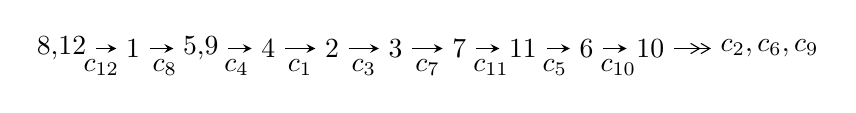
\begin{tikzpicture}[x=23pt, y=7pt]
	% node
	\node (A0) at (-1/8, 0) {8,12};
	\node (A1) at (1, 0) {1};
	\node (A2) at (33/16, 0) {5,9};
	\node (A3) at (25/8, 0) {4};
	\node (A4) at (33/8, 0) {2};
	\node (A5) at (41/8, 0) {3};
	\node (A6) at (49/8, 0) {7};
	\node (A7) at (57/8, 0) {11};
	\node (A8) at (65/8, 0) {6};
	\node (A9) at (73/8, 0) {10};
	\node (C1) at (1/2, -1) {$c_{12}$};
	\node (C2) at (3/2, -1) {$c_{8}$};
	\node (C3) at (21/8, -1) {$c_{4}$};
	\node (C4) at (29/8, -1) {$c_{1}$};
	\node (C5) at (37/8, -1) {$c_{3}$};
	\node (C6) at (45/8, -1) {$c_{7}$};
	\node (C7) at (53/8, -1) {$c_{11}$};
	\node (C8) at (61/8, -1) {$c_{5}$};
	\node (C9) at (69/8, -1) {$c_{10}$};
	\node (A10) at (11, 0) {$c_{2},c_{6},c_{9}$};

	% edge
	\draw[->,>=stealth]	
	(A0) edge (A1) (A1) edge (A2) (A2) edge (A3) (A3) edge (A4) (A4) edge (A5) (A5) edge (A6) (A6) edge (A7) (A7) edge (A8) (A8) edge (A9) ;
	\draw[->>,>={angle 60}]	
	(A9) edge (A10);
\end{tikzpicture} \\ 

\end{tabular} \\

\footnotetext{
The image of knot diagram is generated by the software ``\textbf{Draw programme}" developed by Andrew Bartholomew(\url{http://www.layer8.co.uk/maths/draw/index.htm\#Running-draw}), where we modified some parts for our purpose(\url{https://github.com/CATsTAILs/LinksPainter}).
}\phantom \\ \newline 
\centering \textbf{Ideals for irreducible components\footnotemark of $X_{\text{par}}$} 
 
\begin{align*}
I^u_{1}&=\langle 
-8.37457\times10^{436} u^{125}+9.53003\times10^{436} u^{124}+\cdots+1.35101\times10^{438} b+3.45441\times10^{439},\\
\phantom{I^u_{1}}&\phantom{= \langle  }5.42684\times10^{439} u^{125}-6.41823\times10^{439} u^{124}+\cdots+5.54363\times10^{440} a-3.37566\times10^{442},\\
\phantom{I^u_{1}}&\phantom{= \langle  }u^{126}-2 u^{125}+\cdots-3299 u+1231\rangle \\
I^u_{2}&=\langle 
-16238531 u^{25}+30226626 u^{24}+\cdots+923959 b-38221381,\\
\phantom{I^u_{2}}&\phantom{= \langle  }37676420 u^{25}-76531168 u^{24}+\cdots+923959 a+101309415,\;u^{26}- u^{25}+\cdots- u+1\rangle \\
\\
\end{align*}
\raggedright * 2 irreducible components of $\dim_{\mathbb{C}}=0$, with total 152 representations.\\
\footnotetext{All coefficients of polynomials are rational numbers. But the coefficients are sometimes approximated in decimal forms when there is not enough margin.}
\newpage
\renewcommand{\arraystretch}{1}
\centering \section*{I. $I^u_{1}= \langle -8.37\times10^{436} u^{125}+9.53\times10^{436} u^{124}+\cdots+1.35\times10^{438} b+3.45\times10^{439},\;5.43\times10^{439} u^{125}-6.42\times10^{439} u^{124}+\cdots+5.54\times10^{440} a-3.38\times10^{442},\;u^{126}-2 u^{125}+\cdots-3299 u+1231 \rangle$}
\flushleft \textbf{(i) Arc colorings}\\
\begin{tabular}{m{7pt} m{180pt} m{7pt} m{180pt} }
\flushright $a_{8}=$&$\begin{pmatrix}0\\u\end{pmatrix}$ \\
\flushright $a_{12}=$&$\begin{pmatrix}1\\0\end{pmatrix}$ \\
\flushright $a_{1}=$&$\begin{pmatrix}1\\u^2\end{pmatrix}$ \\
\flushright $a_{5}=$&$\begin{pmatrix}-0.0978932 u^{125}+0.115777 u^{124}+\cdots-60.0039 u+60.8925\\0.0619876 u^{125}-0.0705402 u^{124}+\cdots+50.4110 u-25.5692\end{pmatrix}$ \\
\flushright $a_{9}=$&$\begin{pmatrix}- u\\- u^3+u\end{pmatrix}$ \\
\flushright $a_{4}=$&$\begin{pmatrix}-0.0359056 u^{125}+0.0452365 u^{124}+\cdots-9.59292 u+35.3233\\0.0619876 u^{125}-0.0705402 u^{124}+\cdots+50.4110 u-25.5692\end{pmatrix}$ \\
\flushright $a_{2}=$&$\begin{pmatrix}-0.214789 u^{125}+0.296860 u^{124}+\cdots-474.659 u+353.417\\0.122779 u^{125}-0.161806 u^{124}+\cdots+149.065 u-130.070\end{pmatrix}$ \\
\flushright $a_{3}=$&$\begin{pmatrix}-0.0772666 u^{125}+0.0884009 u^{124}+\cdots-71.4657 u+70.1570\\0.0636737 u^{125}-0.0767534 u^{124}+\cdots+32.6989 u-11.7076\end{pmatrix}$ \\
\flushright $a_{7}=$&$\begin{pmatrix}-0.108594 u^{125}+0.178457 u^{124}+\cdots-259.220 u+200.755\\0.0288267 u^{125}-0.0221697 u^{124}+\cdots+233.565 u-127.968\end{pmatrix}$ \\
\flushright $a_{11}=$&$\begin{pmatrix}0.149451 u^{125}-0.221439 u^{124}+\cdots+127.121 u-131.829\\-0.0290794 u^{125}+0.0255495 u^{124}+\cdots-149.270 u+74.8556\end{pmatrix}$ \\
\flushright $a_{6}=$&$\begin{pmatrix}0.0178159 u^{125}-0.00589056 u^{124}+\cdots+155.501 u-49.6233\\0.0261068 u^{125}-0.222873 u^{124}+\cdots-717.172 u+238.249\end{pmatrix}$ \\
\flushright $a_{10}=$&$\begin{pmatrix}-0.189401 u^{125}+0.179433 u^{124}+\cdots-526.484 u+302.818\\0.115155 u^{125}-0.125900 u^{124}+\cdots+283.633 u-171.090\end{pmatrix}$\\&\end{tabular}
\flushleft \textbf{(ii) Obstruction class $= -1$}\\~\\
\flushleft \textbf{(iii) Cusp Shapes $= -2.46505 u^{125}+6.90651 u^{124}+\cdots+16799.0 u-4389.17$}\\~\\
\newpage\renewcommand{\arraystretch}{1}
\flushleft \textbf{(iv) u-Polynomials at the component}\newline \\
\begin{tabular}{m{50pt}|m{274pt}}
Crossings & \hspace{64pt}u-Polynomials at each crossing \\
\hline $$\begin{aligned}c_{1}\end{aligned}$$&$\begin{aligned}
&u^{126}+9 u^{125}+\cdots+177179 u+46852
\end{aligned}$\\
\hline $$\begin{aligned}c_{2}\end{aligned}$$&$\begin{aligned}
&u^{126}-4 u^{125}+\cdots-21 u+161
\end{aligned}$\\
\hline $$\begin{aligned}c_{3}\end{aligned}$$&$\begin{aligned}
&u^{126}-3 u^{125}+\cdots-1627736 u+491149
\end{aligned}$\\
\hline $$\begin{aligned}c_{4},c_{5},c_{11}\end{aligned}$$&$\begin{aligned}
&u^{126}- u^{125}+\cdots-44 u+1
\end{aligned}$\\
\hline $$\begin{aligned}c_{6},c_{9}\end{aligned}$$&$\begin{aligned}
&u^{126}+4 u^{125}+\cdots+940 u+28
\end{aligned}$\\
\hline $$\begin{aligned}c_{7}\end{aligned}$$&$\begin{aligned}
&u^{126}+11 u^{124}+\cdots+20491 u+4508
\end{aligned}$\\
\hline $$\begin{aligned}c_{8},c_{12}\end{aligned}$$&$\begin{aligned}
&u^{126}-2 u^{125}+\cdots-3299 u+1231
\end{aligned}$\\
\hline $$\begin{aligned}c_{10}\end{aligned}$$&$\begin{aligned}
&u^{126}-6 u^{125}+\cdots-21 u+2
\end{aligned}$\\
\hline
\end{tabular}\\~\\
\newpage\renewcommand{\arraystretch}{1}
\flushleft \textbf{(v) Riley Polynomials at the component}\newline \\
\begin{tabular}{m{50pt}|m{274pt}}
Crossings & \hspace{64pt}Riley Polynomials at each crossing \\
\hline $$\begin{aligned}c_{1}\end{aligned}$$&$\begin{aligned}
&y^{126}-3 y^{125}+\cdots-81214908545 y+2195109904
\end{aligned}$\\
\hline $$\begin{aligned}c_{2}\end{aligned}$$&$\begin{aligned}
&y^{126}-18 y^{125}+\cdots-1745037 y+25921
\end{aligned}$\\
\hline $$\begin{aligned}c_{3}\end{aligned}$$&$\begin{aligned}
&y^{126}+43 y^{125}+\cdots+11414107688058 y+241227340201
\end{aligned}$\\
\hline $$\begin{aligned}c_{4},c_{5},c_{11}\end{aligned}$$&$\begin{aligned}
&y^{126}+129 y^{125}+\cdots-144 y+1
\end{aligned}$\\
\hline $$\begin{aligned}c_{6},c_{9}\end{aligned}$$&$\begin{aligned}
&y^{126}+92 y^{125}+\cdots+2432 y+784
\end{aligned}$\\
\hline $$\begin{aligned}c_{7}\end{aligned}$$&$\begin{aligned}
&y^{126}+22 y^{125}+\cdots+3435910495 y+20322064
\end{aligned}$\\
\hline $$\begin{aligned}c_{8},c_{12}\end{aligned}$$&$\begin{aligned}
&y^{126}-66 y^{125}+\cdots-35934251 y+1515361
\end{aligned}$\\
\hline $$\begin{aligned}c_{10}\end{aligned}$$&$\begin{aligned}
&y^{126}-6 y^{125}+\cdots+743 y+4
\end{aligned}$\\
\hline
\end{tabular}\\~\\
\newpage\flushleft \textbf{(vi) Complex Volumes and Cusp Shapes}
$$\begin{array}{c|c|c}  
\text{Solutions to }I^u_{1}& \I (\text{vol} + \sqrt{-1}CS) & \text{Cusp shape}\\
 \hline 
\begin{aligned}
u &= -0.148848 + 0.997058 I \\
a &= \phantom{-}0.484449 + 0.589301 I \\
b &= -0.699615 - 0.538924 I\end{aligned}
 & -3.08034 - 8.76965 I & \phantom{-0.000000 } 0 \\ \hline\begin{aligned}
u &= -0.148848 - 0.997058 I \\
a &= \phantom{-}0.484449 - 0.589301 I \\
b &= -0.699615 + 0.538924 I\end{aligned}
 & -3.08034 + 8.76965 I & \phantom{-0.000000 } 0 \\ \hline\begin{aligned}
u &= -0.932617 + 0.406689 I \\
a &= \phantom{-}2.39092 + 0.91877 I \\
b &= -0.01303 - 1.43923 I\end{aligned}
 & \phantom{-}7.15726 - 0.43742 I & \phantom{-0.000000 } 0 \\ \hline\begin{aligned}
u &= -0.932617 - 0.406689 I \\
a &= \phantom{-}2.39092 - 0.91877 I \\
b &= -0.01303 + 1.43923 I\end{aligned}
 & \phantom{-}7.15726 + 0.43742 I & \phantom{-0.000000 } 0 \\ \hline\begin{aligned}
u &= \phantom{-}0.139361 + 0.971063 I \\
a &= \phantom{-}0.679799 - 0.430076 I \\
b &= -0.660053 + 0.442878 I\end{aligned}
 & \phantom{-}2.02908 + 3.15648 I & \phantom{-0.000000 } 0 \\ \hline\begin{aligned}
u &= \phantom{-}0.139361 - 0.971063 I \\
a &= \phantom{-}0.679799 + 0.430076 I \\
b &= -0.660053 - 0.442878 I\end{aligned}
 & \phantom{-}2.02908 - 3.15648 I & \phantom{-0.000000 } 0 \\ \hline\begin{aligned}
u &= \phantom{-}0.969622 + 0.329631 I \\
a &= \phantom{-}2.64691 + 0.02661 I \\
b &= -0.03223 + 1.42157 I\end{aligned}
 & \phantom{-}2.85868 + 4.34404 I & \phantom{-0.000000 } 0 \\ \hline\begin{aligned}
u &= \phantom{-}0.969622 - 0.329631 I \\
a &= \phantom{-}2.64691 - 0.02661 I \\
b &= -0.03223 - 1.42157 I\end{aligned}
 & \phantom{-}2.85868 - 4.34404 I & \phantom{-0.000000 } 0 \\ \hline\begin{aligned}
u &= \phantom{-}0.994765 + 0.250646 I \\
a &= \phantom{-}0.051584 - 1.062280 I \\
b &= \phantom{-}0.161305 + 0.726440 I\end{aligned}
 & \phantom{-}0.35382 - 2.73597 I & \phantom{-0.000000 } 0 \\ \hline\begin{aligned}
u &= \phantom{-}0.994765 - 0.250646 I \\
a &= \phantom{-}0.051584 + 1.062280 I \\
b &= \phantom{-}0.161305 - 0.726440 I\end{aligned}
 & \phantom{-}0.35382 + 2.73597 I & \phantom{-0.000000 } 0\\
 \hline 
 \end{array}$$\newpage$$\begin{array}{c|c|c}  
\text{Solutions to }I^u_{1}& \I (\text{vol} + \sqrt{-1}CS) & \text{Cusp shape}\\
 \hline 
\begin{aligned}
u &= -0.943035 + 0.237535 I \\
a &= -0.685926 + 0.121446 I \\
b &= -0.330407 - 0.898944 I\end{aligned}
 & -1.56204 + 0.98621 I & \phantom{-0.000000 } 0 \\ \hline\begin{aligned}
u &= -0.943035 - 0.237535 I \\
a &= -0.685926 - 0.121446 I \\
b &= -0.330407 + 0.898944 I\end{aligned}
 & -1.56204 - 0.98621 I & \phantom{-0.000000 } 0 \\ \hline\begin{aligned}
u &= \phantom{-}0.779175 + 0.581592 I \\
a &= \phantom{-}1.43608 - 2.67401 I \\
b &= -0.01880 + 1.59472 I\end{aligned}
 & \phantom{-}3.92478 - 2.29687 I & \phantom{-0.000000 } 0 \\ \hline\begin{aligned}
u &= \phantom{-}0.779175 - 0.581592 I \\
a &= \phantom{-}1.43608 + 2.67401 I \\
b &= -0.01880 - 1.59472 I\end{aligned}
 & \phantom{-}3.92478 + 2.29687 I & \phantom{-0.000000 } 0 \\ \hline\begin{aligned}
u &= \phantom{-}0.949055 + 0.404563 I \\
a &= -1.71474 + 0.73666 I \\
b &= -0.31857 - 1.54304 I\end{aligned}
 & \phantom{-}7.14144 - 5.30194 I & \phantom{-0.000000 } 0 \\ \hline\begin{aligned}
u &= \phantom{-}0.949055 - 0.404563 I \\
a &= -1.71474 - 0.73666 I \\
b &= -0.31857 + 1.54304 I\end{aligned}
 & \phantom{-}7.14144 + 5.30194 I & \phantom{-0.000000 } 0 \\ \hline\begin{aligned}
u &= -0.919188 + 0.203338 I \\
a &= -1.53946 - 1.04780 I \\
b &= -0.11947 + 1.75078 I\end{aligned}
 & \phantom{-}1.10721 + 0.90973 I & \phantom{-0.000000 } 0 \\ \hline\begin{aligned}
u &= -0.919188 - 0.203338 I \\
a &= -1.53946 + 1.04780 I \\
b &= -0.11947 - 1.75078 I\end{aligned}
 & \phantom{-}1.10721 - 0.90973 I & \phantom{-0.000000 } 0 \\ \hline\begin{aligned}
u &= -0.840820 + 0.395590 I \\
a &= \phantom{-}0.566454 + 0.458444 I \\
b &= \phantom{-}0.522950 - 0.439061 I\end{aligned}
 & -1.69920 + 1.44671 I & \phantom{-0.000000 } 0 \\ \hline\begin{aligned}
u &= -0.840820 - 0.395590 I \\
a &= \phantom{-}0.566454 - 0.458444 I \\
b &= \phantom{-}0.522950 + 0.439061 I\end{aligned}
 & -1.69920 - 1.44671 I & \phantom{-0.000000 } 0\\
 \hline 
 \end{array}$$\newpage$$\begin{array}{c|c|c}  
\text{Solutions to }I^u_{1}& \I (\text{vol} + \sqrt{-1}CS) & \text{Cusp shape}\\
 \hline 
\begin{aligned}
u &= \phantom{-}0.984351 + 0.431623 I \\
a &= -0.313627 + 0.015274 I \\
b &= -0.323201 + 1.073460 I\end{aligned}
 & -3.52157 - 2.16105 I & \phantom{-0.000000 } 0 \\ \hline\begin{aligned}
u &= \phantom{-}0.984351 - 0.431623 I \\
a &= -0.313627 - 0.015274 I \\
b &= -0.323201 - 1.073460 I\end{aligned}
 & -3.52157 + 2.16105 I & \phantom{-0.000000 } 0 \\ \hline\begin{aligned}
u &= \phantom{-}0.189494 + 0.902235 I \\
a &= \phantom{-}0.37826 - 1.91093 I \\
b &= \phantom{-}0.03940 + 1.50859 I\end{aligned}
 & \phantom{-}6.39893 - 2.09183 I & \phantom{-0.000000 } 0 \\ \hline\begin{aligned}
u &= \phantom{-}0.189494 - 0.902235 I \\
a &= \phantom{-}0.37826 + 1.91093 I \\
b &= \phantom{-}0.03940 - 1.50859 I\end{aligned}
 & \phantom{-}6.39893 + 2.09183 I & \phantom{-0.000000 } 0 \\ \hline\begin{aligned}
u &= \phantom{-}1.076520 + 0.119638 I \\
a &= -1.197690 - 0.223514 I \\
b &= -0.426418 + 0.560555 I\end{aligned}
 & -7.01035 - 0.91777 I & \phantom{-0.000000 } 0 \\ \hline\begin{aligned}
u &= \phantom{-}1.076520 - 0.119638 I \\
a &= -1.197690 + 0.223514 I \\
b &= -0.426418 - 0.560555 I\end{aligned}
 & -7.01035 + 0.91777 I & \phantom{-0.000000 } 0 \\ \hline\begin{aligned}
u &= -1.066280 + 0.238950 I \\
a &= -0.44262 + 1.55222 I \\
b &= \phantom{-}0.078194 - 0.586003 I\end{aligned}
 & -3.64530 + 5.96303 I & \phantom{-0.000000 } 0 \\ \hline\begin{aligned}
u &= -1.066280 - 0.238950 I \\
a &= -0.44262 - 1.55222 I \\
b &= \phantom{-}0.078194 + 0.586003 I\end{aligned}
 & -3.64530 - 5.96303 I & \phantom{-0.000000 } 0 \\ \hline\begin{aligned}
u &= \phantom{-}0.836369 + 0.337355 I \\
a &= -1.196980 + 0.497658 I \\
b &= -0.835817 - 0.333023 I\end{aligned}
 & -1.81558 - 5.93479 I & \phantom{-0.000000 } 0 \\ \hline\begin{aligned}
u &= \phantom{-}0.836369 - 0.337355 I \\
a &= -1.196980 - 0.497658 I \\
b &= -0.835817 + 0.333023 I\end{aligned}
 & -1.81558 + 5.93479 I & \phantom{-0.000000 } 0\\
 \hline 
 \end{array}$$\newpage$$\begin{array}{c|c|c}  
\text{Solutions to }I^u_{1}& \I (\text{vol} + \sqrt{-1}CS) & \text{Cusp shape}\\
 \hline 
\begin{aligned}
u &= -1.076530 + 0.257076 I \\
a &= -0.199548 - 0.317015 I \\
b &= \phantom{-}0.93261 + 1.10702 I\end{aligned}
 & -0.95266 + 1.40290 I & \phantom{-0.000000 } 0 \\ \hline\begin{aligned}
u &= -1.076530 - 0.257076 I \\
a &= -0.199548 + 0.317015 I \\
b &= \phantom{-}0.93261 - 1.10702 I\end{aligned}
 & -0.95266 - 1.40290 I & \phantom{-0.000000 } 0 \\ \hline\begin{aligned}
u &= \phantom{-}1.027590 + 0.444521 I \\
a &= -0.752960 + 1.009850 I \\
b &= -0.300262 - 0.004771 I\end{aligned}
 & -6.71965 - 1.59487 I & \phantom{-0.000000 } 0 \\ \hline\begin{aligned}
u &= \phantom{-}1.027590 - 0.444521 I \\
a &= -0.752960 - 1.009850 I \\
b &= -0.300262 + 0.004771 I\end{aligned}
 & -6.71965 + 1.59487 I & \phantom{-0.000000 } 0 \\ \hline\begin{aligned}
u &= -0.666000 + 0.910304 I \\
a &= \phantom{-}0.67044 + 1.74561 I \\
b &= \phantom{-}0.05679 - 1.56434 I\end{aligned}
 & \phantom{-}5.49762 + 3.19311 I & \phantom{-0.000000 } 0 \\ \hline\begin{aligned}
u &= -0.666000 - 0.910304 I \\
a &= \phantom{-}0.67044 - 1.74561 I \\
b &= \phantom{-}0.05679 + 1.56434 I\end{aligned}
 & \phantom{-}5.49762 - 3.19311 I & \phantom{-0.000000 } 0 \\ \hline\begin{aligned}
u &= -1.017980 + 0.497500 I \\
a &= -1.69045 - 0.74925 I \\
b &= -0.30351 + 1.47997 I\end{aligned}
 & \phantom{-}4.08352 + 10.02990 I & \phantom{-0.000000 } 0 \\ \hline\begin{aligned}
u &= -1.017980 - 0.497500 I \\
a &= -1.69045 + 0.74925 I \\
b &= -0.30351 - 1.47997 I\end{aligned}
 & \phantom{-}4.08352 - 10.02990 I & \phantom{-0.000000 } 0 \\ \hline\begin{aligned}
u &= -0.074073 + 1.135800 I \\
a &= \phantom{-}0.25441 - 1.94446 I \\
b &= \phantom{-}0.00690 + 1.46050 I\end{aligned}
 & \phantom{-}6.38693 - 1.83428 I & \phantom{-0.000000 } 0 \\ \hline\begin{aligned}
u &= -0.074073 - 1.135800 I \\
a &= \phantom{-}0.25441 + 1.94446 I \\
b &= \phantom{-}0.00690 - 1.46050 I\end{aligned}
 & \phantom{-}6.38693 + 1.83428 I & \phantom{-0.000000 } 0\\
 \hline 
 \end{array}$$\newpage$$\begin{array}{c|c|c}  
\text{Solutions to }I^u_{1}& \I (\text{vol} + \sqrt{-1}CS) & \text{Cusp shape}\\
 \hline 
\begin{aligned}
u &= \phantom{-}1.000600 + 0.585201 I \\
a &= \phantom{-}1.32389 - 1.27787 I \\
b &= \phantom{-}0.06932 + 1.44806 I\end{aligned}
 & \phantom{-}4.31935 - 3.21172 I & \phantom{-0.000000 } 0 \\ \hline\begin{aligned}
u &= \phantom{-}1.000600 - 0.585201 I \\
a &= \phantom{-}1.32389 + 1.27787 I \\
b &= \phantom{-}0.06932 - 1.44806 I\end{aligned}
 & \phantom{-}4.31935 + 3.21172 I & \phantom{-0.000000 } 0 \\ \hline\begin{aligned}
u &= -0.937234 + 0.690886 I \\
a &= -1.37031 - 2.60421 I \\
b &= -0.066461 + 1.393770 I\end{aligned}
 & -1.99693 + 2.71074 I & \phantom{-0.000000 } 0 \\ \hline\begin{aligned}
u &= -0.937234 - 0.690886 I \\
a &= -1.37031 + 2.60421 I \\
b &= -0.066461 - 1.393770 I\end{aligned}
 & -1.99693 - 2.71074 I & \phantom{-0.000000 } 0 \\ \hline\begin{aligned}
u &= \phantom{-}0.812096 + 0.187109 I \\
a &= -0.04787 - 3.67334 I \\
b &= \phantom{-}0.06270 + 1.56183 I\end{aligned}
 & \phantom{-}3.67919 - 6.70709 I & \phantom{-0.000000 } 0 \\ \hline\begin{aligned}
u &= \phantom{-}0.812096 - 0.187109 I \\
a &= -0.04787 + 3.67334 I \\
b &= \phantom{-}0.06270 - 1.56183 I\end{aligned}
 & \phantom{-}3.67919 + 6.70709 I & \phantom{-0.000000 } 0 \\ \hline\begin{aligned}
u &= -0.829005 + 0.066349 I \\
a &= -1.369970 - 0.124550 I \\
b &= -1.66040 + 0.95864 I\end{aligned}
 & \phantom{-}0.498437 + 0.097480 I & -184.802 + 0. I\phantom{ +0.000000I} \\ \hline\begin{aligned}
u &= -0.829005 - 0.066349 I \\
a &= -1.369970 + 0.124550 I \\
b &= -1.66040 - 0.95864 I\end{aligned}
 & \phantom{-}0.498437 - 0.097480 I & -184.802 + 0. I\phantom{ +0.000000I} \\ \hline\begin{aligned}
u &= \phantom{-}0.318174 + 1.132600 I \\
a &= \phantom{-}0.04738 - 2.15159 I \\
b &= -0.24143 + 1.53554 I\end{aligned}
 & \phantom{-}3.72675 + 12.23680 I & \phantom{-0.000000 } 0 \\ \hline\begin{aligned}
u &= \phantom{-}0.318174 - 1.132600 I \\
a &= \phantom{-}0.04738 + 2.15159 I \\
b &= -0.24143 - 1.53554 I\end{aligned}
 & \phantom{-}3.72675 - 12.23680 I & \phantom{-0.000000 } 0\\
 \hline 
 \end{array}$$\newpage$$\begin{array}{c|c|c}  
\text{Solutions to }I^u_{1}& \I (\text{vol} + \sqrt{-1}CS) & \text{Cusp shape}\\
 \hline 
\begin{aligned}
u &= \phantom{-}0.222388 + 0.775919 I \\
a &= \phantom{-}0.73054 + 1.92549 I \\
b &= \phantom{-}0.087347 - 1.375010 I\end{aligned}
 & \phantom{-}1.24727 + 3.56284 I & \phantom{-0.000000 } 0 \\ \hline\begin{aligned}
u &= \phantom{-}0.222388 - 0.775919 I \\
a &= \phantom{-}0.73054 - 1.92549 I \\
b &= \phantom{-}0.087347 + 1.375010 I\end{aligned}
 & \phantom{-}1.24727 - 3.56284 I & \phantom{-0.000000 } 0 \\ \hline\begin{aligned}
u &= \phantom{-}1.134550 + 0.382624 I \\
a &= -0.915642 + 0.347066 I \\
b &= -0.576662 - 0.305597 I\end{aligned}
 & -3.25311 - 4.39444 I & \phantom{-0.000000 } 0 \\ \hline\begin{aligned}
u &= \phantom{-}1.134550 - 0.382624 I \\
a &= -0.915642 - 0.347066 I \\
b &= -0.576662 + 0.305597 I\end{aligned}
 & -3.25311 + 4.39444 I & \phantom{-0.000000 } 0 \\ \hline\begin{aligned}
u &= -1.159380 + 0.315869 I \\
a &= \phantom{-}0.0490977 + 0.1201230 I \\
b &= -0.100624 - 1.201120 I\end{aligned}
 & -2.96172 - 0.16203 I & \phantom{-0.000000 } 0 \\ \hline\begin{aligned}
u &= -1.159380 - 0.315869 I \\
a &= \phantom{-}0.0490977 - 0.1201230 I \\
b &= -0.100624 + 1.201120 I\end{aligned}
 & -2.96172 + 0.16203 I & \phantom{-0.000000 } 0 \\ \hline\begin{aligned}
u &= -0.479018 + 1.103440 I \\
a &= \phantom{-}0.297343 - 0.252162 I \\
b &= -0.132709 + 0.061105 I\end{aligned}
 & \phantom{-}0.79102 + 2.44530 I & \phantom{-0.000000 } 0 \\ \hline\begin{aligned}
u &= -0.479018 - 1.103440 I \\
a &= \phantom{-}0.297343 + 0.252162 I \\
b &= -0.132709 - 0.061105 I\end{aligned}
 & \phantom{-}0.79102 - 2.44530 I & \phantom{-0.000000 } 0 \\ \hline\begin{aligned}
u &= -0.711681 + 0.329657 I \\
a &= \phantom{-}0.51756 + 2.91327 I \\
b &= \phantom{-}0.06856 - 1.56632 I\end{aligned}
 & \phantom{-}7.95495 + 3.72264 I & \phantom{-0.000000 } 0. - 10.70451 I \\ \hline\begin{aligned}
u &= -0.711681 - 0.329657 I \\
a &= \phantom{-}0.51756 - 2.91327 I \\
b &= \phantom{-}0.06856 + 1.56632 I\end{aligned}
 & \phantom{-}7.95495 - 3.72264 I & \phantom{-0.000000 -}0. + 10.70451 I\\
 \hline 
 \end{array}$$\newpage$$\begin{array}{c|c|c}  
\text{Solutions to }I^u_{1}& \I (\text{vol} + \sqrt{-1}CS) & \text{Cusp shape}\\
 \hline 
\begin{aligned}
u &= -0.409298 + 1.145340 I \\
a &= \phantom{-}0.23193 + 2.10725 I \\
b &= -0.24019 - 1.51287 I\end{aligned}
 & \phantom{-}8.48302 - 6.51011 I & \phantom{-0.000000 } 0 \\ \hline\begin{aligned}
u &= -0.409298 - 1.145340 I \\
a &= \phantom{-}0.23193 - 2.10725 I \\
b &= -0.24019 + 1.51287 I\end{aligned}
 & \phantom{-}8.48302 + 6.51011 I & \phantom{-0.000000 } 0 \\ \hline\begin{aligned}
u &= -1.129780 + 0.471397 I \\
a &= -0.919743 - 0.449485 I \\
b &= -0.627097 + 0.134208 I\end{aligned}
 & -6.34927 + 5.70832 I & \phantom{-0.000000 } 0 \\ \hline\begin{aligned}
u &= -1.129780 - 0.471397 I \\
a &= -0.919743 + 0.449485 I \\
b &= -0.627097 - 0.134208 I\end{aligned}
 & -6.34927 - 5.70832 I & \phantom{-0.000000 } 0 \\ \hline\begin{aligned}
u &= \phantom{-}0.658946 + 0.378164 I \\
a &= \phantom{-}0.250036 + 0.240626 I \\
b &= \phantom{-}0.640273 - 0.579391 I\end{aligned}
 & -1.38842 + 2.68986 I & \phantom{-0.000000 } 0 \\ \hline\begin{aligned}
u &= \phantom{-}0.658946 - 0.378164 I \\
a &= \phantom{-}0.250036 - 0.240626 I \\
b &= \phantom{-}0.640273 + 0.579391 I\end{aligned}
 & -1.38842 - 2.68986 I & \phantom{-0.000000 } 0 \\ \hline\begin{aligned}
u &= \phantom{-}0.458262 + 0.597731 I \\
a &= \phantom{-}0.654853 - 0.467897 I \\
b &= \phantom{-}0.386012 + 0.709668 I\end{aligned}
 & -2.19670 - 1.87960 I & \phantom{-0.000000 -}0. + 4.44403 I \\ \hline\begin{aligned}
u &= \phantom{-}0.458262 - 0.597731 I \\
a &= \phantom{-}0.654853 + 0.467897 I \\
b &= \phantom{-}0.386012 - 0.709668 I\end{aligned}
 & -2.19670 + 1.87960 I & \phantom{-0.000000 } 0. - 4.44403 I \\ \hline\begin{aligned}
u &= -0.146371 + 0.735428 I \\
a &= \phantom{-}0.629678 + 0.135044 I \\
b &= -0.200353 - 0.525626 I\end{aligned}
 & \phantom{-}0.18032 + 2.18521 I & \phantom{-}5.35102 - 2.23079 I \\ \hline\begin{aligned}
u &= -0.146371 - 0.735428 I \\
a &= \phantom{-}0.629678 - 0.135044 I \\
b &= -0.200353 + 0.525626 I\end{aligned}
 & \phantom{-}0.18032 - 2.18521 I & \phantom{-}5.35102 + 2.23079 I\\
 \hline 
 \end{array}$$\newpage$$\begin{array}{c|c|c}  
\text{Solutions to }I^u_{1}& \I (\text{vol} + \sqrt{-1}CS) & \text{Cusp shape}\\
 \hline 
\begin{aligned}
u &= -0.131562 + 0.731311 I \\
a &= \phantom{-}0.53826 + 1.50162 I \\
b &= -0.633873 - 0.485988 I\end{aligned}
 & -3.20346 + 4.20633 I & -1.42742 - 4.24409 I \\ \hline\begin{aligned}
u &= -0.131562 - 0.731311 I \\
a &= \phantom{-}0.53826 - 1.50162 I \\
b &= -0.633873 + 0.485988 I\end{aligned}
 & -3.20346 - 4.20633 I & -1.42742 + 4.24409 I \\ \hline\begin{aligned}
u &= -0.476604 + 0.567281 I \\
a &= -0.00364 - 1.54332 I \\
b &= \phantom{-}0.19968 + 1.54911 I\end{aligned}
 & \phantom{-}5.68339 - 5.76173 I & \phantom{-}4.03620 + 1.96765 I \\ \hline\begin{aligned}
u &= -0.476604 - 0.567281 I \\
a &= -0.00364 + 1.54332 I \\
b &= \phantom{-}0.19968 - 1.54911 I\end{aligned}
 & \phantom{-}5.68339 + 5.76173 I & \phantom{-}4.03620 - 1.96765 I \\ \hline\begin{aligned}
u &= -1.219270 + 0.331553 I \\
a &= \phantom{-}0.106622 + 0.357014 I \\
b &= \phantom{-}0.962536 - 0.062103 I\end{aligned}
 & -2.78023 + 0.97303 I & \phantom{-0.000000 } 0 \\ \hline\begin{aligned}
u &= -1.219270 - 0.331553 I \\
a &= \phantom{-}0.106622 - 0.357014 I \\
b &= \phantom{-}0.962536 + 0.062103 I\end{aligned}
 & -2.78023 - 0.97303 I & \phantom{-0.000000 } 0 \\ \hline\begin{aligned}
u &= \phantom{-}0.651889 + 0.337481 I \\
a &= -0.42475 + 1.61434 I \\
b &= \phantom{-}0.16202 - 1.63051 I\end{aligned}
 & \phantom{-}8.12960 + 1.97140 I & \phantom{-}4.04397 + 3.29297 I \\ \hline\begin{aligned}
u &= \phantom{-}0.651889 - 0.337481 I \\
a &= -0.42475 - 1.61434 I \\
b &= \phantom{-}0.16202 + 1.63051 I\end{aligned}
 & \phantom{-}8.12960 - 1.97140 I & \phantom{-}4.04397 - 3.29297 I \\ \hline\begin{aligned}
u &= \phantom{-}0.596740 + 1.116480 I \\
a &= \phantom{-}0.62338 - 1.94608 I \\
b &= -0.30543 + 1.41182 I\end{aligned}
 & \phantom{-}5.05717 - 0.14156 I & \phantom{-0.000000 } 0 \\ \hline\begin{aligned}
u &= \phantom{-}0.596740 - 1.116480 I \\
a &= \phantom{-}0.62338 + 1.94608 I \\
b &= -0.30543 - 1.41182 I\end{aligned}
 & \phantom{-}5.05717 + 0.14156 I & \phantom{-0.000000 } 0\\
 \hline 
 \end{array}$$\newpage$$\begin{array}{c|c|c}  
\text{Solutions to }I^u_{1}& \I (\text{vol} + \sqrt{-1}CS) & \text{Cusp shape}\\
 \hline 
\begin{aligned}
u &= -1.251670 + 0.248282 I \\
a &= -0.942174 - 0.163311 I \\
b &= -0.546637 + 0.467593 I\end{aligned}
 & -7.24377 + 4.41221 I & \phantom{-0.000000 } 0 \\ \hline\begin{aligned}
u &= -1.251670 - 0.248282 I \\
a &= -0.942174 + 0.163311 I \\
b &= -0.546637 - 0.467593 I\end{aligned}
 & -7.24377 - 4.41221 I & \phantom{-0.000000 } 0 \\ \hline\begin{aligned}
u &= \phantom{-}1.162380 + 0.531161 I \\
a &= -1.98603 + 1.00024 I \\
b &= -0.172096 - 1.386380 I\end{aligned}
 & -1.51459 - 8.43395 I & \phantom{-0.000000 } 0 \\ \hline\begin{aligned}
u &= \phantom{-}1.162380 - 0.531161 I \\
a &= -1.98603 - 1.00024 I \\
b &= -0.172096 + 1.386380 I\end{aligned}
 & -1.51459 + 8.43395 I & \phantom{-0.000000 } 0 \\ \hline\begin{aligned}
u &= \phantom{-}1.207860 + 0.421033 I \\
a &= -0.0178337 - 0.0720407 I \\
b &= \phantom{-}1.008340 - 0.506746 I\end{aligned}
 & -6.96323 - 8.27018 I & \phantom{-0.000000 } 0 \\ \hline\begin{aligned}
u &= \phantom{-}1.207860 - 0.421033 I \\
a &= -0.0178337 + 0.0720407 I \\
b &= \phantom{-}1.008340 + 0.506746 I\end{aligned}
 & -6.96323 + 8.27018 I & \phantom{-0.000000 } 0 \\ \hline\begin{aligned}
u &= -1.189610 + 0.583725 I \\
a &= -0.489387 - 0.424237 I \\
b &= -0.265791 + 0.205094 I\end{aligned}
 & -1.73251 + 3.52502 I & \phantom{-0.000000 } 0 \\ \hline\begin{aligned}
u &= -1.189610 - 0.583725 I \\
a &= -0.489387 + 0.424237 I \\
b &= -0.265791 - 0.205094 I\end{aligned}
 & -1.73251 - 3.52502 I & \phantom{-0.000000 } 0 \\ \hline\begin{aligned}
u &= -1.227660 + 0.501625 I \\
a &= -1.55719 - 0.96114 I \\
b &= -0.16818 + 1.45759 I\end{aligned}
 & \phantom{-}2.51802 + 6.99481 I & \phantom{-0.000000 } 0 \\ \hline\begin{aligned}
u &= -1.227660 - 0.501625 I \\
a &= -1.55719 + 0.96114 I \\
b &= -0.16818 - 1.45759 I\end{aligned}
 & \phantom{-}2.51802 - 6.99481 I & \phantom{-0.000000 } 0\\
 \hline 
 \end{array}$$\newpage$$\begin{array}{c|c|c}  
\text{Solutions to }I^u_{1}& \I (\text{vol} + \sqrt{-1}CS) & \text{Cusp shape}\\
 \hline 
\begin{aligned}
u &= -1.220020 + 0.537137 I \\
a &= \phantom{-}0.55937 + 1.32266 I \\
b &= \phantom{-}0.639267 - 0.912827 I\end{aligned}
 & -6.20401 + 0.67249 I & \phantom{-0.000000 } 0 \\ \hline\begin{aligned}
u &= -1.220020 - 0.537137 I \\
a &= \phantom{-}0.55937 - 1.32266 I \\
b &= \phantom{-}0.639267 + 0.912827 I\end{aligned}
 & -6.20401 - 0.67249 I & \phantom{-0.000000 } 0 \\ \hline\begin{aligned}
u &= -0.641115 + 0.181165 I \\
a &= \phantom{-}2.68375 - 1.34030 I \\
b &= -0.151706 - 0.040572 I\end{aligned}
 & -2.20245 - 3.80287 I & \phantom{-}2.77639 - 4.05015 I \\ \hline\begin{aligned}
u &= -0.641115 - 0.181165 I \\
a &= \phantom{-}2.68375 + 1.34030 I \\
b &= -0.151706 + 0.040572 I\end{aligned}
 & -2.20245 + 3.80287 I & \phantom{-}2.77639 + 4.05015 I \\ \hline\begin{aligned}
u &= -0.178617 + 0.633748 I \\
a &= \phantom{-}0.424577 - 0.096385 I \\
b &= \phantom{-}0.544428 + 0.225863 I\end{aligned}
 & -3.65130 - 1.45525 I & -4.73147 + 3.01385 I \\ \hline\begin{aligned}
u &= -0.178617 - 0.633748 I \\
a &= \phantom{-}0.424577 + 0.096385 I \\
b &= \phantom{-}0.544428 - 0.225863 I\end{aligned}
 & -3.65130 + 1.45525 I & -4.73147 - 3.01385 I \\ \hline\begin{aligned}
u &= \phantom{-}1.240540 + 0.526594 I \\
a &= \phantom{-}0.386316 - 0.877754 I \\
b &= \phantom{-}0.932489 + 0.626542 I\end{aligned}
 & -1.39198 - 8.45006 I & \phantom{-0.000000 } 0 \\ \hline\begin{aligned}
u &= \phantom{-}1.240540 - 0.526594 I \\
a &= \phantom{-}0.386316 + 0.877754 I \\
b &= \phantom{-}0.932489 - 0.626542 I\end{aligned}
 & -1.39198 + 8.45006 I & \phantom{-0.000000 } 0 \\ \hline\begin{aligned}
u &= \phantom{-}1.342150 + 0.132858 I \\
a &= \phantom{-}0.110083 - 0.685341 I \\
b &= \phantom{-}0.160826 + 1.248210 I\end{aligned}
 & \phantom{-}0.74225 - 2.91628 I & \phantom{-0.000000 } 0 \\ \hline\begin{aligned}
u &= \phantom{-}1.342150 - 0.132858 I \\
a &= \phantom{-}0.110083 + 0.685341 I \\
b &= \phantom{-}0.160826 - 1.248210 I\end{aligned}
 & \phantom{-}0.74225 + 2.91628 I & \phantom{-0.000000 } 0\\
 \hline 
 \end{array}$$\newpage$$\begin{array}{c|c|c}  
\text{Solutions to }I^u_{1}& \I (\text{vol} + \sqrt{-1}CS) & \text{Cusp shape}\\
 \hline 
\begin{aligned}
u &= -1.260140 + 0.554115 I \\
a &= \phantom{-}0.525111 + 0.894267 I \\
b &= \phantom{-}0.862357 - 0.634721 I\end{aligned}
 & -6.5214 + 14.2956 I & \phantom{-0.000000 } 0 \\ \hline\begin{aligned}
u &= -1.260140 - 0.554115 I \\
a &= \phantom{-}0.525111 - 0.894267 I \\
b &= \phantom{-}0.862357 + 0.634721 I\end{aligned}
 & -6.5214 - 14.2956 I & \phantom{-0.000000 } 0 \\ \hline\begin{aligned}
u &= \phantom{-}1.348730 + 0.318201 I \\
a &= \phantom{-}0.068972 - 0.170369 I \\
b &= \phantom{-}0.759504 - 0.238728 I\end{aligned}
 & -8.13778 + 4.10129 I & \phantom{-0.000000 } 0 \\ \hline\begin{aligned}
u &= \phantom{-}1.348730 - 0.318201 I \\
a &= \phantom{-}0.068972 + 0.170369 I \\
b &= \phantom{-}0.759504 + 0.238728 I\end{aligned}
 & -8.13778 - 4.10129 I & \phantom{-0.000000 } 0 \\ \hline\begin{aligned}
u &= \phantom{-}1.341980 + 0.347451 I \\
a &= -1.31337 + 0.64564 I \\
b &= -0.16379 - 1.51215 I\end{aligned}
 & -0.69437 - 6.95691 I & \phantom{-0.000000 } 0 \\ \hline\begin{aligned}
u &= \phantom{-}1.341980 - 0.347451 I \\
a &= -1.31337 - 0.64564 I \\
b &= -0.16379 + 1.51215 I\end{aligned}
 & -0.69437 + 6.95691 I & \phantom{-0.000000 } 0 \\ \hline\begin{aligned}
u &= \phantom{-}1.215820 + 0.687867 I \\
a &= \phantom{-}0.98021 - 1.68467 I \\
b &= \phantom{-}0.38806 + 1.55320 I\end{aligned}
 & \phantom{-}2.80725 - 6.41201 I & \phantom{-0.000000 } 0 \\ \hline\begin{aligned}
u &= \phantom{-}1.215820 - 0.687867 I \\
a &= \phantom{-}0.98021 + 1.68467 I \\
b &= \phantom{-}0.38806 - 1.55320 I\end{aligned}
 & \phantom{-}2.80725 + 6.41201 I & \phantom{-0.000000 } 0 \\ \hline\begin{aligned}
u &= \phantom{-}1.325560 + 0.486468 I \\
a &= -0.620531 + 0.161435 I \\
b &= -0.283598 - 0.388858 I\end{aligned}
 & -4.28613 - 6.83274 I & \phantom{-0.000000 } 0 \\ \hline\begin{aligned}
u &= \phantom{-}1.325560 - 0.486468 I \\
a &= -0.620531 - 0.161435 I \\
b &= -0.283598 + 0.388858 I\end{aligned}
 & -4.28613 + 6.83274 I & \phantom{-0.000000 } 0\\
 \hline 
 \end{array}$$\newpage$$\begin{array}{c|c|c}  
\text{Solutions to }I^u_{1}& \I (\text{vol} + \sqrt{-1}CS) & \text{Cusp shape}\\
 \hline 
\begin{aligned}
u &= -1.24621 + 0.67949 I \\
a &= \phantom{-}1.21880 + 1.58383 I \\
b &= \phantom{-}0.31321 - 1.57749 I\end{aligned}
 & \phantom{-}5.7485 + 12.9840 I & \phantom{-0.000000 } 0 \\ \hline\begin{aligned}
u &= -1.24621 - 0.67949 I \\
a &= \phantom{-}1.21880 - 1.58383 I \\
b &= \phantom{-}0.31321 + 1.57749 I\end{aligned}
 & \phantom{-}5.7485 - 12.9840 I & \phantom{-0.000000 } 0 \\ \hline\begin{aligned}
u &= \phantom{-}1.26837 + 0.66057 I \\
a &= \phantom{-}1.33678 - 1.54106 I \\
b &= \phantom{-}0.29857 + 1.58276 I\end{aligned}
 & \phantom{-}0.7099 - 18.5946 I & \phantom{-0.000000 } 0 \\ \hline\begin{aligned}
u &= \phantom{-}1.26837 - 0.66057 I \\
a &= \phantom{-}1.33678 + 1.54106 I \\
b &= \phantom{-}0.29857 - 1.58276 I\end{aligned}
 & \phantom{-}0.7099 + 18.5946 I & \phantom{-0.000000 } 0 \\ \hline\begin{aligned}
u &= \phantom{-}0.60781 + 1.34059 I \\
a &= -0.11147 + 1.98504 I \\
b &= -0.02176 - 1.42990 I\end{aligned}
 & \phantom{-}5.96691 - 2.85688 I & \phantom{-0.000000 } 0 \\ \hline\begin{aligned}
u &= \phantom{-}0.60781 - 1.34059 I \\
a &= -0.11147 - 1.98504 I \\
b &= -0.02176 + 1.42990 I\end{aligned}
 & \phantom{-}5.96691 + 2.85688 I & \phantom{-0.000000 } 0 \\ \hline\begin{aligned}
u &= \phantom{-}1.23071 + 0.81446 I \\
a &= -1.03642 + 1.64382 I \\
b &= -0.07588 - 1.44304 I\end{aligned}
 & \phantom{-}3.78807 - 4.69844 I & \phantom{-0.000000 } 0 \\ \hline\begin{aligned}
u &= \phantom{-}1.23071 - 0.81446 I \\
a &= -1.03642 - 1.64382 I \\
b &= -0.07588 + 1.44304 I\end{aligned}
 & \phantom{-}3.78807 + 4.69844 I & \phantom{-0.000000 } 0 \\ \hline\begin{aligned}
u &= -1.50987 + 0.09187 I \\
a &= -0.014556 - 0.815056 I \\
b &= \phantom{-}0.214295 + 1.367810 I\end{aligned}
 & -3.12537 - 7.53337 I & \phantom{-0.000000 } 0 \\ \hline\begin{aligned}
u &= -1.50987 - 0.09187 I \\
a &= -0.014556 + 0.815056 I \\
b &= \phantom{-}0.214295 - 1.367810 I\end{aligned}
 & -3.12537 + 7.53337 I & \phantom{-0.000000 } 0\\
 \hline 
 \end{array}$$\newpage$$\begin{array}{c|c|c}  
\text{Solutions to }I^u_{1}& \I (\text{vol} + \sqrt{-1}CS) & \text{Cusp shape}\\
 \hline 
\begin{aligned}
u &= \phantom{-}0.427169 + 0.181956 I \\
a &= \phantom{-}2.69543 - 0.61581 I \\
b &= -0.240674 + 0.130137 I\end{aligned}
 & \phantom{-}1.79440 + 0.02427 I & \phantom{-}7.84012 + 1.45955 I \\ \hline\begin{aligned}
u &= \phantom{-}0.427169 - 0.181956 I \\
a &= \phantom{-}2.69543 + 0.61581 I \\
b &= -0.240674 - 0.130137 I\end{aligned}
 & \phantom{-}1.79440 - 0.02427 I & \phantom{-}7.84012 - 1.45955 I \\ \hline\begin{aligned}
u &= -1.42925 + 0.64803 I \\
a &= -1.01971 - 1.14875 I \\
b &= -0.09841 + 1.48811 I\end{aligned}
 & \phantom{-}1.98063 + 8.26315 I & \phantom{-0.000000 } 0 \\ \hline\begin{aligned}
u &= -1.42925 - 0.64803 I \\
a &= -1.01971 + 1.14875 I \\
b &= -0.09841 - 1.48811 I\end{aligned}
 & \phantom{-}1.98063 - 8.26315 I & \phantom{-0.000000 } 0 \\ \hline\begin{aligned}
u &= -0.050278 + 0.411683 I \\
a &= \phantom{-}0.550036 + 0.242277 I \\
b &= \phantom{-}0.297186 - 0.449903 I\end{aligned}
 & -0.135812 + 1.155040 I & -1.96188 - 5.19114 I \\ \hline\begin{aligned}
u &= -0.050278 - 0.411683 I \\
a &= \phantom{-}0.550036 - 0.242277 I \\
b &= \phantom{-}0.297186 + 0.449903 I\end{aligned}
 & -0.135812 - 1.155040 I & -1.96188 + 5.19114 I\\
 \hline 
 \end{array}$$\newpage\newpage\renewcommand{\arraystretch}{1}
\centering \section*{II. $I^u_{2}= \langle -1.62\times10^{7} u^{25}+3.02\times10^{7} u^{24}+\cdots+9.24\times10^{5} b-3.82\times10^{7},\;3.77\times10^{7} u^{25}-7.65\times10^{7} u^{24}+\cdots+9.24\times10^{5} a+1.01\times10^{8},\;u^{26}- u^{25}+\cdots- u+1 \rangle$}
\flushleft \textbf{(i) Arc colorings}\\
\begin{tabular}{m{7pt} m{180pt} m{7pt} m{180pt} }
\flushright $a_{8}=$&$\begin{pmatrix}0\\u\end{pmatrix}$ \\
\flushright $a_{12}=$&$\begin{pmatrix}1\\0\end{pmatrix}$ \\
\flushright $a_{1}=$&$\begin{pmatrix}1\\u^2\end{pmatrix}$ \\
\flushright $a_{5}=$&$\begin{pmatrix}-40.7772 u^{25}+82.8296 u^{24}+\cdots+258.260 u-109.647\\17.5749 u^{25}-32.7143 u^{24}+\cdots-103.573 u+41.3670\end{pmatrix}$ \\
\flushright $a_{9}=$&$\begin{pmatrix}- u\\- u^3+u\end{pmatrix}$ \\
\flushright $a_{4}=$&$\begin{pmatrix}-23.2022 u^{25}+50.1154 u^{24}+\cdots+154.688 u-68.2801\\17.5749 u^{25}-32.7143 u^{24}+\cdots-103.573 u+41.3670\end{pmatrix}$ \\
\flushright $a_{2}=$&$\begin{pmatrix}42.0013 u^{25}-97.8731 u^{24}+\cdots-341.143 u+160.014\\-4.79559 u^{25}+0.0230584 u^{24}+\cdots+18.0952 u+6.60502\end{pmatrix}$ \\
\flushright $a_{3}=$&$\begin{pmatrix}-23.2022 u^{25}+49.1154 u^{24}+\cdots+153.688 u-67.2801\\17.5749 u^{25}-32.7143 u^{24}+\cdots-103.573 u+41.3670\end{pmatrix}$ \\
\flushright $a_{7}=$&$\begin{pmatrix}-66.2314 u^{25}+77.8533 u^{24}+\cdots+243.213 u-58.3855\\0.592913 u^{25}-4.06860 u^{24}+\cdots-24.5921 u+16.7433\end{pmatrix}$ \\
\flushright $a_{11}=$&$\begin{pmatrix}-27.2660 u^{25}+35.2638 u^{24}+\cdots+139.740 u-31.9295\\0.268166 u^{25}+5.87467 u^{24}+\cdots+23.0432 u-20.7456\end{pmatrix}$ \\
\flushright $a_{6}=$&$\begin{pmatrix}67.9432 u^{25}-97.9002 u^{24}+\cdots-299.466 u+99.3720\\-40.8380 u^{25}+63.9847 u^{24}+\cdots+160.509 u-48.8588\end{pmatrix}$ \\
\flushright $a_{10}=$&$\begin{pmatrix}-25.6943 u^{25}+58.6272 u^{24}+\cdots+148.725 u-86.1828\\42.2036 u^{25}-63.4743 u^{24}+\cdots-168.537 u+53.7065\end{pmatrix}$\\&\end{tabular}
\flushleft \textbf{(ii) Obstruction class $= 1$}\\~\\
\flushleft \textbf{(iii) Cusp Shapes $= \frac{149866747}{923959} u^{25}-\frac{337930009}{923959} u^{24}+\cdots-\frac{651165116}{923959} u+\frac{351073846}{923959}$}\\~\\
\newpage\renewcommand{\arraystretch}{1}
\flushleft \textbf{(iv) u-Polynomials at the component}\newline \\
\begin{tabular}{m{50pt}|m{274pt}}
Crossings & \hspace{64pt}u-Polynomials at each crossing \\
\hline $$\begin{aligned}c_{1}\end{aligned}$$&$\begin{aligned}
&u^{26}-12 u^{25}+\cdots-36 u+7
\end{aligned}$\\
\hline $$\begin{aligned}c_{2}\end{aligned}$$&$\begin{aligned}
&u^{26}- u^{25}+\cdots- u+1
\end{aligned}$\\
\hline $$\begin{aligned}c_{3}\end{aligned}$$&$\begin{aligned}
&u^{26}+2 u^{25}+\cdots+10 u^2+1
\end{aligned}$\\
\hline $$\begin{aligned}c_{4},c_{5}\end{aligned}$$&$\begin{aligned}
&u^{26}+2 u^{25}+\cdots+2 u+1
\end{aligned}$\\
\hline $$\begin{aligned}c_{6}\end{aligned}$$&$\begin{aligned}
&u^{26}+5 u^{25}+\cdots+16 u+4
\end{aligned}$\\
\hline $$\begin{aligned}c_{7}\end{aligned}$$&$\begin{aligned}
&u^{26}+u^{25}+\cdots-38 u+13
\end{aligned}$\\
\hline $$\begin{aligned}c_{8}\end{aligned}$$&$\begin{aligned}
&u^{26}+u^{25}+\cdots+u+1
\end{aligned}$\\
\hline $$\begin{aligned}c_{9}\end{aligned}$$&$\begin{aligned}
&u^{26}-5 u^{25}+\cdots-16 u+4
\end{aligned}$\\
\hline $$\begin{aligned}c_{10}\end{aligned}$$&$\begin{aligned}
&u^{26}- u^{25}+\cdots+3 u+1
\end{aligned}$\\
\hline $$\begin{aligned}c_{11}\end{aligned}$$&$\begin{aligned}
&u^{26}-2 u^{25}+\cdots-2 u+1
\end{aligned}$\\
\hline $$\begin{aligned}c_{12}\end{aligned}$$&$\begin{aligned}
&u^{26}- u^{25}+\cdots- u+1
\end{aligned}$\\
\hline
\end{tabular}\\~\\
\newpage\renewcommand{\arraystretch}{1}
\flushleft \textbf{(v) Riley Polynomials at the component}\newline \\
\begin{tabular}{m{50pt}|m{274pt}}
Crossings & \hspace{64pt}Riley Polynomials at each crossing \\
\hline $$\begin{aligned}c_{1}\end{aligned}$$&$\begin{aligned}
&y^{26}+12 y^{25}+\cdots-1044 y+49
\end{aligned}$\\
\hline $$\begin{aligned}c_{2}\end{aligned}$$&$\begin{aligned}
&y^{26}-7 y^{25}+\cdots-7 y+1
\end{aligned}$\\
\hline $$\begin{aligned}c_{3}\end{aligned}$$&$\begin{aligned}
&y^{26}+6 y^{25}+\cdots+20 y+1
\end{aligned}$\\
\hline $$\begin{aligned}c_{4},c_{5},c_{11}\end{aligned}$$&$\begin{aligned}
&y^{26}+28 y^{25}+\cdots-2 y+1
\end{aligned}$\\
\hline $$\begin{aligned}c_{6},c_{9}\end{aligned}$$&$\begin{aligned}
&y^{26}+19 y^{25}+\cdots+48 y+16
\end{aligned}$\\
\hline $$\begin{aligned}c_{7}\end{aligned}$$&$\begin{aligned}
&y^{26}+13 y^{25}+\cdots+402 y+169
\end{aligned}$\\
\hline $$\begin{aligned}c_{8},c_{12}\end{aligned}$$&$\begin{aligned}
&y^{26}-11 y^{25}+\cdots-21 y+1
\end{aligned}$\\
\hline $$\begin{aligned}c_{10}\end{aligned}$$&$\begin{aligned}
&y^{26}-3 y^{25}+\cdots+77 y+1
\end{aligned}$\\
\hline
\end{tabular}\\~\\
\newpage\flushleft \textbf{(vi) Complex Volumes and Cusp Shapes}
$$\begin{array}{c|c|c}  
\text{Solutions to }I^u_{2}& \I (\text{vol} + \sqrt{-1}CS) & \text{Cusp shape}\\
 \hline 
\begin{aligned}
u &= \phantom{-}0.960119 + 0.265758 I \\
a &= -0.865721 + 0.373600 I \\
b &= -0.084741 + 1.101490 I\end{aligned}
 & -4.25818 - 1.08751 I & -6.83580 + 0.03087 I \\ \hline\begin{aligned}
u &= \phantom{-}0.960119 - 0.265758 I \\
a &= -0.865721 - 0.373600 I \\
b &= -0.084741 - 1.101490 I\end{aligned}
 & -4.25818 + 1.08751 I & -6.83580 - 0.03087 I \\ \hline\begin{aligned}
u &= -1.054200 + 0.354405 I \\
a &= -0.135482 + 0.199760 I \\
b &= -0.470597 - 0.875277 I\end{aligned}
 & -1.43501 + 1.97726 I & -0.64126 - 4.43069 I \\ \hline\begin{aligned}
u &= -1.054200 - 0.354405 I \\
a &= -0.135482 - 0.199760 I \\
b &= -0.470597 + 0.875277 I\end{aligned}
 & -1.43501 - 1.97726 I & -0.64126 + 4.43069 I \\ \hline\begin{aligned}
u &= -1.007140 + 0.507041 I \\
a &= -1.14054 - 1.37225 I \\
b &= -0.208869 + 0.631292 I\end{aligned}
 & -5.86020 + 2.09818 I & -2.54692 - 5.18070 I \\ \hline\begin{aligned}
u &= -1.007140 - 0.507041 I \\
a &= -1.14054 + 1.37225 I \\
b &= -0.208869 - 0.631292 I\end{aligned}
 & -5.86020 - 2.09818 I & -2.54692 + 5.18070 I \\ \hline\begin{aligned}
u &= -0.444960 + 1.086040 I \\
a &= -0.162395 + 0.208043 I \\
b &= \phantom{-}0.237746 - 0.229386 I\end{aligned}
 & \phantom{-}0.78338 + 2.62725 I & -0.4991 - 24.3792 I \\ \hline\begin{aligned}
u &= -0.444960 - 1.086040 I \\
a &= -0.162395 - 0.208043 I \\
b &= \phantom{-}0.237746 + 0.229386 I\end{aligned}
 & \phantom{-}0.78338 - 2.62725 I & -0.4991 + 24.3792 I \\ \hline\begin{aligned}
u &= -0.803695 + 0.076489 I \\
a &= \phantom{-}1.395030 + 0.140155 I \\
b &= \phantom{-}1.39037 - 0.91387 I\end{aligned}
 & \phantom{-}0.528666 + 0.091290 I & \phantom{-}82.3409 + 7.4167 I \\ \hline\begin{aligned}
u &= -0.803695 - 0.076489 I \\
a &= \phantom{-}1.395030 - 0.140155 I \\
b &= \phantom{-}1.39037 + 0.91387 I\end{aligned}
 & \phantom{-}0.528666 - 0.091290 I & \phantom{-}82.3409 - 7.4167 I\\
 \hline 
 \end{array}$$\newpage$$\begin{array}{c|c|c}  
\text{Solutions to }I^u_{2}& \I (\text{vol} + \sqrt{-1}CS) & \text{Cusp shape}\\
 \hline 
\begin{aligned}
u &= \phantom{-}0.462571 + 1.101380 I \\
a &= -0.47701 + 2.15047 I \\
b &= \phantom{-}0.21416 - 1.45525 I\end{aligned}
 & \phantom{-}4.91648 - 0.52982 I & \phantom{-}0.63138 + 6.27014 I \\ \hline\begin{aligned}
u &= \phantom{-}0.462571 - 1.101380 I \\
a &= -0.47701 - 2.15047 I \\
b &= \phantom{-}0.21416 + 1.45525 I\end{aligned}
 & \phantom{-}4.91648 + 0.52982 I & \phantom{-}0.63138 - 6.27014 I \\ \hline\begin{aligned}
u &= \phantom{-}1.201810 + 0.366511 I \\
a &= -0.708024 - 0.242130 I \\
b &= -0.418255 - 0.082920 I\end{aligned}
 & -4.97637 - 6.17880 I & -6.64629 + 6.66766 I \\ \hline\begin{aligned}
u &= \phantom{-}1.201810 - 0.366511 I \\
a &= -0.708024 + 0.242130 I \\
b &= -0.418255 + 0.082920 I\end{aligned}
 & -4.97637 + 6.17880 I & -6.64629 - 6.66766 I \\ \hline\begin{aligned}
u &= \phantom{-}0.608019 + 1.127160 I \\
a &= \phantom{-}0.36868 - 1.86104 I \\
b &= \phantom{-}0.04734 + 1.50210 I\end{aligned}
 & \phantom{-}6.89482 - 3.51056 I & \phantom{-}8.78887 + 6.66749 I \\ \hline\begin{aligned}
u &= \phantom{-}0.608019 - 1.127160 I \\
a &= \phantom{-}0.36868 + 1.86104 I \\
b &= \phantom{-}0.04734 - 1.50210 I\end{aligned}
 & \phantom{-}6.89482 + 3.51056 I & \phantom{-}8.78887 - 6.66749 I \\ \hline\begin{aligned}
u &= \phantom{-}0.675393 + 0.069978 I \\
a &= \phantom{-}1.79298 + 1.77615 I \\
b &= \phantom{-}0.417235 - 0.297568 I\end{aligned}
 & -2.42704 + 4.22616 I & -5.58020 - 10.10054 I \\ \hline\begin{aligned}
u &= \phantom{-}0.675393 - 0.069978 I \\
a &= \phantom{-}1.79298 - 1.77615 I \\
b &= \phantom{-}0.417235 + 0.297568 I\end{aligned}
 & -2.42704 - 4.22616 I & -5.58020 + 10.10054 I \\ \hline\begin{aligned}
u &= -1.317960 + 0.417827 I \\
a &= -1.35617 - 0.48271 I \\
b &= -0.12420 + 1.45986 I\end{aligned}
 & \phantom{-}0.42159 + 7.99851 I & -0.97759 - 7.43929 I \\ \hline\begin{aligned}
u &= -1.317960 - 0.417827 I \\
a &= -1.35617 + 0.48271 I \\
b &= -0.12420 - 1.45986 I\end{aligned}
 & \phantom{-}0.42159 - 7.99851 I & -0.97759 + 7.43929 I\\
 \hline 
 \end{array}$$\newpage$$\begin{array}{c|c|c}  
\text{Solutions to }I^u_{2}& \I (\text{vol} + \sqrt{-1}CS) & \text{Cusp shape}\\
 \hline 
\begin{aligned}
u &= \phantom{-}1.275590 + 0.594910 I \\
a &= -1.11717 + 1.27143 I \\
b &= -0.22257 - 1.44164 I\end{aligned}
 & \phantom{-}1.82130 - 5.71135 I & -1.05320 + 3.00564 I \\ \hline\begin{aligned}
u &= \phantom{-}1.275590 - 0.594910 I \\
a &= -1.11717 - 1.27143 I \\
b &= -0.22257 + 1.44164 I\end{aligned}
 & \phantom{-}1.82130 + 5.71135 I & -1.05320 - 3.00564 I \\ \hline\begin{aligned}
u &= -0.578294 + 0.025496 I \\
a &= \phantom{-}1.87129 - 4.02484 I \\
b &= \phantom{-}0.10678 + 1.53450 I\end{aligned}
 & \phantom{-}4.01860 - 5.98752 I & \phantom{-}1.67587 + 1.84987 I \\ \hline\begin{aligned}
u &= -0.578294 - 0.025496 I \\
a &= \phantom{-}1.87129 + 4.02484 I \\
b &= \phantom{-}0.10678 - 1.53450 I\end{aligned}
 & \phantom{-}4.01860 + 5.98752 I & \phantom{-}1.67587 - 1.84987 I \\ \hline\begin{aligned}
u &= \phantom{-}0.522750 + 0.238445 I \\
a &= \phantom{-}1.53454 - 2.56686 I \\
b &= \phantom{-}0.11560 + 1.56506 I\end{aligned}
 & \phantom{-}7.79662 - 3.07854 I & \phantom{-}3.34333 + 0.16527 I \\ \hline\begin{aligned}
u &= \phantom{-}0.522750 - 0.238445 I \\
a &= \phantom{-}1.53454 + 2.56686 I \\
b &= \phantom{-}0.11560 - 1.56506 I\end{aligned}
 & \phantom{-}7.79662 + 3.07854 I & \phantom{-}3.34333 - 0.16527 I\\
 \hline 
 \end{array}$$\newpage
\newpage\renewcommand{\arraystretch}{1}
\centering \section*{ III. u-Polynomials}
\begin{tabular}{m{50pt}|m{274pt}}
Crossings & \hspace{64pt}u-Polynomials at each crossing \\
\hline $$\begin{aligned}c_{1}\end{aligned}$$&$\begin{aligned}
&(u^{26}-12 u^{25}+\cdots-36 u+7)(u^{126}+9 u^{125}+\cdots+177179 u+46852)
\end{aligned}$\\
\hline $$\begin{aligned}c_{2}\end{aligned}$$&$\begin{aligned}
&(u^{26}- u^{25}+\cdots- u+1)(u^{126}-4 u^{125}+\cdots-21 u+161)
\end{aligned}$\\
\hline $$\begin{aligned}c_{3}\end{aligned}$$&$\begin{aligned}
&(u^{26}+2 u^{25}+\cdots+10 u^2+1)(u^{126}-3 u^{125}+\cdots-1627736 u+491149)
\end{aligned}$\\
\hline $$\begin{aligned}c_{4},c_{5}\end{aligned}$$&$\begin{aligned}
&(u^{26}+2 u^{25}+\cdots+2 u+1)(u^{126}- u^{125}+\cdots-44 u+1)
\end{aligned}$\\
\hline $$\begin{aligned}c_{6}\end{aligned}$$&$\begin{aligned}
&(u^{26}+5 u^{25}+\cdots+16 u+4)(u^{126}+4 u^{125}+\cdots+940 u+28)
\end{aligned}$\\
\hline $$\begin{aligned}c_{7}\end{aligned}$$&$\begin{aligned}
&(u^{26}+u^{25}+\cdots-38 u+13)(u^{126}+11 u^{124}+\cdots+20491 u+4508)
\end{aligned}$\\
\hline $$\begin{aligned}c_{8}\end{aligned}$$&$\begin{aligned}
&(u^{26}+u^{25}+\cdots+u+1)(u^{126}-2 u^{125}+\cdots-3299 u+1231)
\end{aligned}$\\
\hline $$\begin{aligned}c_{9}\end{aligned}$$&$\begin{aligned}
&(u^{26}-5 u^{25}+\cdots-16 u+4)(u^{126}+4 u^{125}+\cdots+940 u+28)
\end{aligned}$\\
\hline $$\begin{aligned}c_{10}\end{aligned}$$&$\begin{aligned}
&(u^{26}- u^{25}+\cdots+3 u+1)(u^{126}-6 u^{125}+\cdots-21 u+2)
\end{aligned}$\\
\hline $$\begin{aligned}c_{11}\end{aligned}$$&$\begin{aligned}
&(u^{26}-2 u^{25}+\cdots-2 u+1)(u^{126}- u^{125}+\cdots-44 u+1)
\end{aligned}$\\
\hline $$\begin{aligned}c_{12}\end{aligned}$$&$\begin{aligned}
&(u^{26}- u^{25}+\cdots- u+1)(u^{126}-2 u^{125}+\cdots-3299 u+1231)
\end{aligned}$\\
\hline
\end{tabular}\newpage\renewcommand{\arraystretch}{1}
\centering \section*{ IV. Riley Polynomials}
\begin{tabular}{m{50pt}|m{274pt}}
Crossings & \hspace{64pt}Riley Polynomials at each crossing \\
\hline $$\begin{aligned}c_{1}\end{aligned}$$&$\begin{aligned}
&(y^{26}+12 y^{25}+\cdots-1044 y+49)\\
&\cdot(y^{126}-3 y^{125}+\cdots-81214908545 y+2195109904)
\end{aligned}$\\
\hline $$\begin{aligned}c_{2}\end{aligned}$$&$\begin{aligned}
&(y^{26}-7 y^{25}+\cdots-7 y+1)(y^{126}-18 y^{125}+\cdots-1745037 y+25921)
\end{aligned}$\\
\hline $$\begin{aligned}c_{3}\end{aligned}$$&$\begin{aligned}
&(y^{26}+6 y^{25}+\cdots+20 y+1)\\
&\cdot(y^{126}+43 y^{125}+\cdots+11414107688058 y+241227340201)
\end{aligned}$\\
\hline $$\begin{aligned}c_{4},c_{5},c_{11}\end{aligned}$$&$\begin{aligned}
&(y^{26}+28 y^{25}+\cdots-2 y+1)(y^{126}+129 y^{125}+\cdots-144 y+1)
\end{aligned}$\\
\hline $$\begin{aligned}c_{6},c_{9}\end{aligned}$$&$\begin{aligned}
&(y^{26}+19 y^{25}+\cdots+48 y+16)(y^{126}+92 y^{125}+\cdots+2432 y+784)
\end{aligned}$\\
\hline $$\begin{aligned}c_{7}\end{aligned}$$&$\begin{aligned}
&(y^{26}+13 y^{25}+\cdots+402 y+169)\\
&\cdot(y^{126}+22 y^{125}+\cdots+3435910495 y+20322064)
\end{aligned}$\\
\hline $$\begin{aligned}c_{8},c_{12}\end{aligned}$$&$\begin{aligned}
&(y^{26}-11 y^{25}+\cdots-21 y+1)\\
&\cdot(y^{126}-66 y^{125}+\cdots-35934251 y+1515361)
\end{aligned}$\\
\hline $$\begin{aligned}c_{10}\end{aligned}$$&$\begin{aligned}
&(y^{26}-3 y^{25}+\cdots+77 y+1)(y^{126}-6 y^{125}+\cdots+743 y+4)
\end{aligned}$\\
\hline
\end{tabular}
\vskip 2pc
\end{document}